\documentclass[8pt]{extarticle}
\usepackage{geometry}
% \usepackage{showframe}

\geometry{
    a4paper, 
    margin=0.5in
}

\usepackage{graphicx} % Required for inserting images
\usepackage{amsmath}
\usepackage{amsfonts}
\usepackage{preamble}
\usepackage{multicol}
\usepackage{lipsum}
\usepackage[framemethod=TikZ]{mdframed}
\usepackage{thmboxes}
\usepackage{float}

\begin{document}
\section{\huge Algebra}
\begin{multicols}{2}
\subsection{Functions and Symmetries}

\begin{dfn}[Functions]{thm:functions}{0.1.1}
A function $f:X\to Y$ is called
\renewcommand\labelitemi{\tiny$\bullet$}
\begin{itemize}
    \setlength\itemsep{0em}
    \item \textit{injective} if $f(x_{1}) = f(x_{2}) \implies x_{1} = x_{{2}}$
    \item \textit{surjective} if for every $y\in Y,\, \exists x\in X$ s.t. $f(x) = y$
    \item \textit{bijective} if it is both injective and surjective
\end{itemize}
% \begin{figure}[H]
%     \centering
%     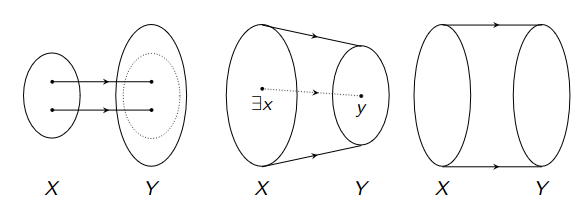
\includegraphics[width=\linewidth]{images/functions.png}
% \end{figure}
\end{dfn}

\begin{dfn}[Graph Isomorphisms]{thm:graph-iso}{1.1.3}
    An \textbf{isomorphism} between two graphs is a \textit{bijection} between them that preserves all edges. More precisely, if $\Gamma_{1}$ and $\Gamma_{2}$ are graphs, with sets of vertices $V_{1}$ and $V_{2}$ respectively, then an isomorphism from $\Gamma_{1}$ and $\Gamma_{2}$ is a bijection
    $$f : V_{1}\to V_{2}$$
    such that $f(v_{1})$ and $f(v_{2})$ are joined by an edge if and only if $v_{1}$ and $v_{2}$ are also joined by an edge.
    We say that $\Gamma_{1}$ and $\Gamma_{2}$ are \textit{isomorphic} if there exists an isomorphism $f:\Gamma_{1}\to\Gamma_{2}$
\end{dfn}

\begin{dfn}[Symmetry]{thm:symmetry}{1.1.9}
    A \textbf{symmetry} of a graph is an \textit{isomorphism} from the graph to itself, i.e. if the set of vertices is V, then the symmetry is a bijection $f:V\to V$ that preserves edges. That is, a symmetry is a bijection $f:V\to V$ such that $f(v_{1})$ and $f(v_{2})$ are joined by an edge if and only if $v_{1}$ and $v_{2}$ are joined by an edge.
\end{dfn}

\subsection{Groups}

\begin{dfn}[Groups]{thm:group-def}{1.2.3}
    For an operation $\ast$, We say a non-empty set G is a \textbf{group} under $\ast$ if the following four axioms hold:
    \renewcommand\labelitemi{\tiny$\bullet$}
    \begin{itemize}
        \setlength\itemsep{0em}
        \item \textbf{G1 - Closure:} $\ast$ is a binary operation on G, that is $a\ast b \in G$ for all $a,b\in G$.
        \item \textbf{G2 - Associativity:} $(a\ast b) \ast c =a\ast(b\ast c)$ for all $a,b,c\in G$
        \item \textbf{G3 - Identity:} There exists an \textit{identity} element of $G$ such that $e\ast g = g\ast e = e$ for all $g\in G$.
        \item \textbf{G4 - Inverse:} Every element $g\in G$ has an *inverse* $g^{-1}$ such that $g\ast g^{-1}=g^{-1}\ast g = e$
    \end{itemize}
\end{dfn}

\begin{dfn}[Abelian Group]{thm:abelian}{1.2.6}
    The definition of a group doesn't require that $a\ast b = b\ast a$.
    We say that a group is \textbf{abelian} or \textbf{commutative} if $a\ast b = b\ast a$ for every $a,b\in G$. We say that $a$ \textit{commutes} with $b$, or that $a$ and $b$ \textit{commute}
\end{dfn}

\begin{dfn}[Order of a Group]{thm:group-order}{2.1.?}
    The \textbf{order} of a finite group, written $\lvert G \rvert$, is the number of elements in $G$.
    If $G$ is infinite we say that $\lvert G \rvert = \infty$, or the order of $G$ is infinite.
\end{dfn}
% TODO: Examples of groups
% Dihedral, Symmetric, Product Group, Sets of numbers

\subsection{Subgroups}

\begin{dfn}[Subgroups]{thm:subgroup-def}{2.1.1}
    Let $G$ be a group. We say that a non-empty subset $H$ of $G$ is a \textbf{subgroup} of $G$ if $H$ itself is a group (under the operation from $G$). We write $H\le G$ if $H$ is a subgroup of $G$. If $H\ne G$, we write $H<G$ and say $H$ is a proper subgroup
\end{dfn}

\begin{thm}[Subgroup Test]{thm:subgroup-test}{2.1.3}
    $H\subseteq G$ is a subgroup of $G$ if and only if:
    \renewcommand\labelitemi{\tiny$\bullet$}
    \begin{itemize}
        \setlength\itemsep{0em}
        \item \textbf{S1:} $H$ is not empty
        \item \textbf{S2:} If $h,k\in H$ then $h\ast k\in H$
        \item \textbf{S3:} If $h\in H$ then $h^{-1}\in H$
    \end{itemize}
    Alternative test for subgroups:
    \renewcommand\labelitemi{\tiny$\bullet$}
    \begin{itemize}
        \setlength\itemsep{0em}
        \item $\widetilde{S1}$: $H$ is not empty.
        \item $\widetilde{S2}$: If $h,k\in H$ then $h*k^{-1}\in H$
    \end{itemize}
\end{thm}
\lipsum[1-12]

\end{multicols}

\end{document}